%%% compile it with pdflatex
\documentclass[a4paper]{article}
\usepackage[T1]{fontenc}
\usepackage[utf8]{inputenc}
\usepackage{lmodern}
\usepackage{fancybox}
\usepackage{graphicx}

\begin{document}

\title{2APL: A Practical Programming Language and Platform for Multi-agent Systems}
 
\author{Beltran Borja Fiz, Fabrizio De Santis, Marcos Gabarda\\
\small \texttt{\{beltran.borja.fiz, fabrizio.de.santis, marcos.gabarda\}@est.fib.upc.edu}\\
\\
Multi-Agent Systems Course\\
Master in Artificial Intelligence\\
Universitat Polit\`ecnica de Catalunya}
\date{\today}

\newenvironment{fminipage}%
  {\begin{Sbox}\begin{minipage}}%
  {\end{minipage}\end{Sbox}\fbox{\TheSbox}}


\maketitle

\tableofcontents

\section{Introduction} %%%%%%% BORJA HERE

Borja here: introduce 2apl with history

\section{2APL Language} %%%%%%% BORJA HERE

Introduce prolog + blockworld example
\\
2APL distinguishes itself from other agent-oriented programming
languages by realizing an effective integration of declarative and
imperative style programming.
The declarative style programming supports the implementation of
the mental state of agents allowing them to reason about their
mental states and update them accordingly.
The imperative style programming supports the implementation of
processes allowing programming constructs to implement both the
flow of control as well as mechanisms such as procedure call,
recursion, plan revision, and interface to existing imperative
programming languages.


\subsection{Syntax and operational semantics} %%%%%%% FABRIZIO HERE

There are two distinguished set of programming constructs for defining either a multi-agent system or individual agents.

\subsubsection{Multi-agent system specification} %%%%%%% FABRIZIO HERE

A multi-agent system is specified by a set of couples specifying each agent of the society and a set of environments they have access to. A formal specification of a multi-agent system is provided in Figure~\ref{}. An example for the blockworld environment described above is provided in ~\ref{} where the agent \texttt{harry} and \texttt{sally} are defined both having access to the \texttt{blockworld} environment.

\begin{figure}[htbp]
\begin{verbatim}
<MAS_Prog>     := ( <agentname> ``:'' <filename> [<int>]
                   [<environments>] )+
<agentname>    := <ident>
<filename>     := <ident>``.2apl''
<environments> := ``@''<ident> (``,'' <ident>)*
\end{verbatim}
\end{figure}

\begin{figure}[htbp]
\begin{verbatim}
harry : harry.2apl @blockworld
sally : sally.2apl @blockworld
\end{verbatim}
\end{figure}

\subsubsection{Individual agent specification} %%%%%%% FABRIZIO HERE

2APL agents are implemented in terms of:
	\begin{itemize}
		\item beliefs	
		\item goals	
		\item actions
		\item plans
		\item events
		\item 3 kind of different practical reasoning rules for
			\begin{itemize}
				\item Generating plans for achieving goals
				\item Processing events and messages
				\item Handling and repairing failed plans
			\end{itemize}			
	\end{itemize}

The beliefs, goals, plans and reasoning rules form the \emph{mental states} of the 2APL agent.

Agent can observe an environment either:
	\begin{itemize}
	  \item actively by means of a sense action
	  \item passively by means of events generated by the environment
	\end{itemize}

\begin{verbatim}
	<Agent_Prog> := ( ``Include:'' <ident>
	                | ``BeliefUpdates:'' <BelUpSpec>
	                | ``Beliefs:'' <belief> 
	                | ``Goals:'' <goals> 
	                | ``Plans:'' <plans>
	                | ``PG-rules:'' <pgrules>
	                | ``PC-rules:'' <pcrules>
	                | ``PR-rules:'' <prrules>
	                )*
\end{verbatim}

The basic elements of the language are:
\begin{itemize}
		\item \texttt{<atom>}: Prolog like atomic formula starting with a lowercase letter
		\begin{itemize}
			\item Prolog formulas
		\end{itemize}
		\vskip 2.0ex
		\item \texttt{<Atom>}: Prolog like atomic formula starting with a capital letter
		\begin{itemize}
			\item Function names
		\end{itemize}
		
		\break
		
		\item \texttt{<ground\_atom>}: grounded atomic formula
		\begin{itemize}
			\item Prolog formulas that does not contain any variables
		\end{itemize}
		\vskip 2.0ex
		\item \texttt{<Var>}: string with a capital letter
		\begin{itemize}
			\item Variables
		\end{itemize}
		\vskip 2.0ex
		\item \texttt{<ident>}: string with a lowercase letter
	\end{itemize}

A 2APL agent has \emph{beliefs} and \emph{goals} that may change during the execution

	\begin{itemize}
		\item Beliefs are contained into a \emph{belief base} and they are related to:
			\begin{itemize}
				\item The environment
				\item Other agents
			\end{itemize}
		\item Goals are contained into a \emph{goal base}
	\end{itemize}
	
Rationality principle: if an agent believes a certain fact, then it can not purse that fact as a goal	
	\begin{itemize}
		\item If an agent modifies its belief base, then its goal base may require a modification
	\end{itemize}

\begin{verbatim}
	``Beliefs:'' <belief>
	
	<belief>   := ( <ground_atom> ``.''
	              | <atom> ``:-'' <literals> ``.'' 
	              )+
	<literals> := <literal> (``,'' <literal>)*
	<literal>  := ( <atom> 
	              | ``not'' <atom>
	              )
	\end{verbatim}

\begin{itemize}
		\item Actually, a belief base is a Prolog program
		\begin{itemize}
			\item Each belief is a Prolog fact or rule
			\item All facts are assumed to be grounded
		\end{itemize}
\end{itemize}

\begin{verbatim}
	Beliefs:
	       bomb(3,4).
	       clean(blockWorld) :- not bomb(X,Y), not carry(bomb).
	\end{verbatim}

\begin{verbatim}
	``Goals:'' <goals>
	
	<goals> := <goal> ( ``,'' <goal> )*
	<goal>  := <ground_atom> ( ``and'' <ground_atom> )*
	\end{verbatim}

Each goal expression is a conjunction of ground atoms. 
	
	\begin{verbatim}
	Goals:
	     clean(blockWorld)
	\end{verbatim}
	
	\begin{itemize}
		\item Having ``\texttt{a and b}'' is different than having ``\texttt{a, b}''
		\item Goal base is a list such that the goals are ordered
	\end{itemize}

	A 2APL agent needs to act in order to achieve its goals.

	There are 6 types of basic actions:
	
	\begin{enumerate}
		\item Belief base update action
		\item Communication action
		\item External action
		\item Abstract action
		\item Test actions
		\item Goal dynamic actions
	\end{enumerate}
	
	\begin{verbatim}
	<baction> = ( ``skip'' | <beliefupdate>
	            | <sendaction> | <externalaction> 
	            | <abstractaction> | <test>
	            | <adoptgoal> | <dropgoal>
	            )
	\end{verbatim}

Belief update action
	
\begin{verbatim}
	``BeliefUpdates:'' <BelUpSpec>
	
	<BelUpSpec>    := (
	                  ``{'' <belquery> ``}''
	                      <beliefupdate>
	                  ``{'' <literals> ``}''
	                  )+
	<belquery>     := ( ``true'' 
	                  | <belquery> ``and'' <belquery>
	                  | <belquery> ``or'' <belquery>
	                  | ``('' <belquery> ``)''
	                  | <literal>
	                  )
	<beliefupdate> := <Atom>
\end{verbatim}

\begin{verbatim}
	Updates the belief base using precondition-delete-add formalism.

	BeliefUpdates:
	  { bomb(X,Y) }       RemoveBomb(X,Y) { not bomb(X,Y) }
	  { true }            AddBomb(X,Y)    { bomb(X,Y) }
	  { carry(bomb) }     Drop()          { not carry(bomb) }
	  { not carry(bomb) } PickUp()        { carry(bomb) }
\end{verbatim}

	\begin{itemize}
		\item The specification of belief update actions does not change during agent execution
		\item After the execution of the action, the post-condition is entailed by the belief base
	\end{itemize}

	A communication action passes a message to another agent.

	\begin{verbatim}
	<sendaction> := ``send('' <iv> ``,'' <iv> ``,''
	                        [ <iv> ``,'' <iv> ``,'' ]  <atom> ``)''  
	<iv>         := <ident> | <Var>
	\end{verbatim}

	\begin{verbatim}
	send(Receiver, Performative, Language, Ontology, Content)
	or
	send(Receiver, Performative, Content)
	\end{verbatim}

	\begin{verbatim}
	send(harry, inform, La, On, bombAt(X1,Y1))
	\end{verbatim}

	An external action is \emph{supposed} to change the state of an external environment
	
	\begin{itemize}
		\item Effects of actions are assumed to be determined by the environment
		\item A sense action needs to be performed to determine an effect
	\end{itemize}	
	
	\begin{verbatim}
	<externalaction> := ``@'' <ident> ``('' <atom> ``,'' <Var> ``)''
	\end{verbatim}

	\begin{verbatim}
	@Env(ActionName, Return, Time-out)
	\end{verbatim}

	\begin{verbatim}
	@blockworld(east(), L)
	\end{verbatim}

	\begin{verbatim}
	<abstractlaction> := <atom>
	\end{verbatim}

	\begin{itemize}
		\item It is similar to a procedure call
		\item It substitutes the current execution of a plan with the instantiation of another plan
	\end{itemize}

	Test actions are query expressions used to check if an agent can derive certain beliefs and goals from its bases.

	\begin{verbatim}
	<test>      := ( ``B('' <belquery> ``)'' 
	               | ``G('' <goalquery> ``)''
	               | <test> ``&'' <test>
	               )
	<goalquery> := ( ``true'' 
	               | <goalquery> ``and'' <goalquery>
	               | <goalquery> ``or'' <goalquery>
	               | ``('' <goalquery> ``)''
	               | <atom>
	               )
	\end{verbatim}

	\begin{verbatim}
	p(a)                       // belief
	...
	q(b)                       // goal
	...
	B(p(X)) & G(q(X))          // fails	
	B(p(X)) & G(q(Y) or r(X))  // success by {X/a, Y/b}
	\end{verbatim}

	They are used to adopt and drop goals to and from an agent's goal base.

	\begin{verbatim}
	<adoptgoal> := ( ``adopta('' <goalvar> ``)''
	               | ``adoptz('' <goalvar> ``)''
	               )
	<dropgoal>  := ( ``dropgoal('' <goalvar> ``)''
	               | ``dropsubgoals('' <goalvar> ``)''
	               | ``dropsupergoals('' <goalvar> ``)''
	               )
	<goalvar>   := ( <atom> | ``not'' <atom> )
	\end{verbatim}

It is programmer task to ensure that the variables are instantiated before the actions are executed.

	\begin{verbatim}
	// Goal base
	a(1)
	a(1) and b(1)
	a(1) and b(1) and c(1)

	...

	dropgoal(a(1) and b(1))       // drops a(1) and b(1)
	dropsubgoal(a(1) and b(1))    // drops a(1), a(1) and b(1)
	dropsupergoal(a(1) and b(1))  // drops a(1) and b(1), a(1) and b(1) and c(1)
	\end{verbatim}

	In order to reach its goals, a 2APL agent adopts \emph{plans}.

	A plan consists of basic actions that can be composed by using different operators:
	\begin{itemize}
		\item sequence operator
		\item conditional choice operators
		\item conditional iteration operator
		\item atomic operator for plans that must be executed atomically
	\end{itemize}	

	An agent can have different plans at the same time.

	\begin{verbatim}
	<plan>         := ( <baction> | <sequenceplan>
	                  | <ifplan> | <whileplan>
	                  | <atomicplan>
	                  )
	<sequenceplan> := <plan> ``;'' <plan>
	<ifplan>       := ``if'' <test> ``then'' <scopeplan>
	                 [``else'' <scopeplan>]
	<scopeplan>    := ``{'' <plan ``}''
	<whileplan>    := ``while'' <text> ``do'' <scopeplan>
	<atomicplan>   := ``['' <plan> ``]''
	\end{verbatim}

	The plans of a 2APL agent are implemented by its plan base.
	
	\begin{verbatim}
	Plans: <plans>

	<plans> := <plan> ( ``,'' <plan> )*
	\end{verbatim}

	Initial plan base:

	\begin{verbatim}
	Plans:

	B(start(X,Y)) ; @blockworld(enter(X, Y, blue), L)
	\end{verbatim}	

	3 \emph{practical} reasoning rules are used for generating plans.	

	\begin{enumerate}
		\item Planning goal rules (PG rules)
		\item Procedural rules    (PC rules)
		\item Plan repair rules   (PR rules)
	\end{enumerate}

	They are used to generate plans starting from certain beliefs and goals.
	\begin{verbatim}
	``PG-rules:'' <pgrules>
	
	<pgrules> := <pgrule>+
	<pgrule>  := [<goalquery>] ``<-'' <belquery> ``|'' <plan>
	\end{verbatim}

	\begin{verbatim}
	PG-rules:
	clean(blockWorld) <- bomb(X, Y) | { 
	goto(X, Y);                  // abstract action
	@blockworld(pickup(), L1);   // external action
	PickUp();                    // belief update action
	RemoveBomb(X, Y);

	goto(0, 0);
	@blockworld(drop(), L2);
	Drop();
	}
	\end{verbatim}

	They are used to generate plans as a response to:

	\begin{enumerate}
		\item the execution of abstract actions
		\item the reception of
		\begin{itemize}
			\item messages from other agents
			\item events generated by the external environment or internally
		\end{itemize}
	\end{enumerate}

	\begin{verbatim}
	``PC-rules:'' <pcrules>
	
	<pcrules> = <pcrule>+
	<pcrule> = <atom> ``<-'' <belquery> ``|'' <plan>
	\end{verbatim}

	A PC rule is applied iif the belief condition is entailed by the belief base.

	\begin{verbatim}
	PC-rules:
	goto(X, Y) <- true | {
	  @blockworld(sensePosition(), POS);
	  B(POS = [A,B]);
	  if B(A > X) then {
	     @blockworld( west(), L);
	     goto(X, Y);
	  } else if B(A < X) then {
	     @blockworld( east(), L);
	     goto(X, Y);
	  } else if B(B > Y) then {
	     @blockworld( north(), L);
	     goto(X, Y);
	  } else if B(B < Y) then {
	    @blockworld(south(), L);
	    goto(X, Y);
	  }
	}
	\end{verbatim}

	\begin{verbatim}
	message(sally, inform, La, On, bombAt(X, Y)) <- true | {
	  if B(not bomb(A, B)) then { 
	    AddBomb(X, Y);
	    adoptz(clean(blockWorld));
	  } else { 
	    AddBomb(X, Y);
	  }
	}
	\end{verbatim}

	They are used to replace a plan whose execution has failed.

	\begin{verbatim}
	``PR-rules:'' <prrules>

	<prrules>      := <prrule>+
	<pcrule>       := <planvar> ``<-'' <belquery> ``|'' <planvar>
	<planvar>      := ( <plan>
	                  | <Var>
	                  | ``if'' <test> ``then'' <scopeplanvar>
	                   [``else'' <scopeplanvar>]
	                  | ``while'' <test> ``do'' <scopeplanvar> 
	                  | <planvar> ``;'' <planvar>
	                  )
	<scopeplanvar> := ``{'' <planvar> ``}''
	\end{verbatim}

	It can be applied iif:
	\begin{enumerate}
		\item the execution of a plan fails
		\item there is rule matching the failed action
		\item the belief query expression is derivable from the agent's belief base
	\end{enumerate}

 	\begin{verbatim}
 	PR-rules:
 	@blockworld(pickup(), L) ; REST <- true | { 
	    @blockworld(sensePosition(), POS);
	    B(POS = [X, Y]);     // test action	
	    RemoveBomb(X, Y);    // belief update action
 	}
 	\end{verbatim}

	\texttt{REST}: the rest of the original plan is dropped.

	When the execution of a plan fails?

	It depends on the type of the action
	\begin{itemize}
		\item Belief update action
			\begin{itemize}
				\item  It is not specified or the pre-condition is not entailed by the belief base
			\end{itemize}
		\item Abstract action
			\begin{itemize}
				\item There is no applicable procedural rule 
			\end{itemize}
		\item External action
			\begin{itemize}
				\item The environment throws an \texttt{ExternalActionFailedException}
				\item The agent has no access to the environment
				\item The actions is not defined in the environment
			\end{itemize}
		\item Test action 
			\begin{itemize}
				\item The test expression is no derivable from the belief or goal bases
			\end{itemize}
		\item Goal adopt action
			\begin{itemize}
				\item The goal is already entailed by the belief base
				\item The goal to be adopted is not ground
			\end{itemize}
		\item Atomic plan
			\begin{itemize}
				\item If one of its actions fails
			\end{itemize}
	\end{itemize}

	The execution of all other actions will be always successful.

\subsubsection{Programming the environment} %%%%%%% FABRIZIO HERE

2APL environment can be any Java class implementing the \emph{environment interface}

	It contains the following methods:

	\begin{itemize}
		\item \texttt{addAgent(String name)}
		\item \texttt{removeAgent(String name)}
	\end{itemize}

	Any external action \texttt{@env($a_1, \ldots, a_n$, R)} is translated into a call to a method $m$ with arguments $a_1, \ldots, a_n$ in environment $env$

	\begin{verbatim}
	public Term move(String agent, String direction)
	   throws ExternalActionFailedException {
   	   
	   if (direction.equals("north") { moveNorth(); }
   	   else if (direction.equals("east") {moveEast(); }
   	   else if (direction.equals("south") {moveSouth(); }
   	   else if (direction.equals("west") {moveWest(); }
   	   else throw
	        new ExternalActionFailedException("Unknown direction");

   	   return getPositionTerm();
	}
	\end{verbatim}

	\begin{itemize}
	\item \emph{Events} are used to pass information from environments to agents

	The programmer can decide when and which information from the environment pass to agents using:
	
	\texttt{notifyEvent(AF event, String ... agents)}

	\item The \emph{exception} are used to inform that an action has failed.
	\end{itemize}

	Different agents may \emph{share} certain initial beliefs, goals, plans, belief updates, and practical reasoning rules.

	\begin{verbatim}
	Include: person.2apl    // implements goto(X,Y)
	\end{verbatim}

\subsection{Formal Semantics} %%%%%%% MARCOS HERE

Marcos here

\subsection{Deliberation Cycle} %%%%%%% FABRIZIO HERE

The deliberation cycle is used to determine what the agent should do next

	\begin{center}
 		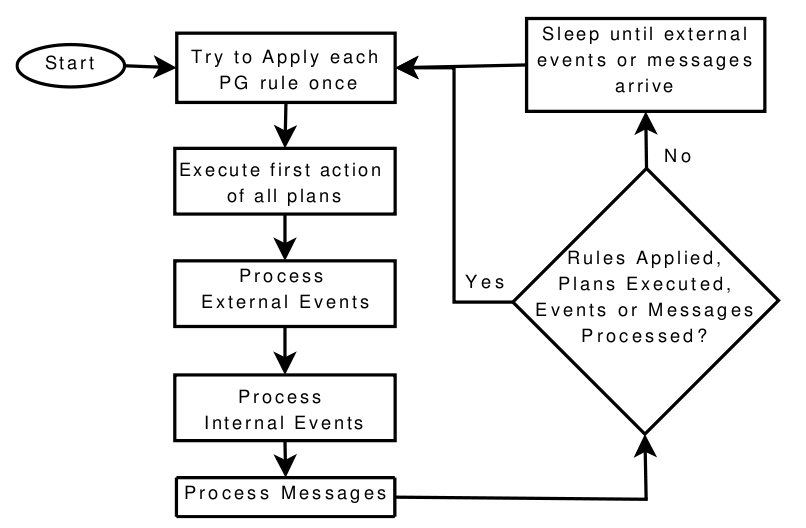
\includegraphics[keepaspectratio,scale=0.3]{fig/rcycle.png}
	\end{center}

	Properties:
	\begin{enumerate}
		\item If the execution of a plan fails, then the plan will either be repaired in the same deliberation cycle or get re-executed in the next deliberation cycle
		\item If the first action fails and there is no plan repair rule for it, then the failed plan may be successfully executed in the next deliberation cycle
	\end{enumerate}

\section{2APL Platform and Tools} %%%%%%% BORJA+MARCOS HERE

Borja+Marcos here

\section{Conclusion} %%%%%%% BORJA HERE

Borja here: conclusion + connecting with other alternatives (jadex etc)

\section{Bibliography}
\nocite{*}
\bibliographystyle{plain}
\bibliography{2apl-doc}

\end{document}
